% 2002 年春季京蒙皖理卷第 15 题：正方形折叠成直二面角
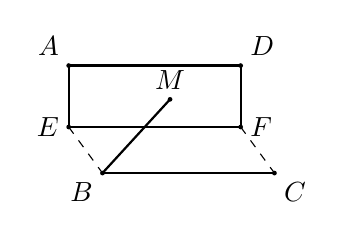
\begin{tikzpicture}[scale=0.78]
  \coordinate (A) at (0,2);
  \coordinate (D) at (2.8,2);
  \coordinate (E) at (0,1);
  \coordinate (F) at (2.8,1);
  \coordinate (B) at (0.55,0.25);
  \coordinate (C) at (3.35,0.25);
  \coordinate (M) at (1.65,1.45);

  \draw[thick] (A)--(D)--(F)--(E)--cycle;
  \draw[thick] (E)--(F);
  \draw[thick] (B)--(C);
  \draw[dashed] (E)--(B) (F)--(C);
  \draw[thick] (B)--(M);

  \fill (A) circle (1.1pt) node[above left] {$A$};
  \fill (D) circle (1.1pt) node[above right] {$D$};
  \fill (E) circle (1.1pt) node[left] {$E$};
  \fill (F) circle (1.1pt) node[right] {$F$};
  \fill (B) circle (1.1pt) node[below left] {$B$};
  \fill (C) circle (1.1pt) node[below right] {$C$};
  \fill (M) circle (1.1pt) node[above] {$M$};
\end{tikzpicture}
